\newpage

\section{Структура двусвязного графа}

\subsection{Одиночные множества и части двусвязного графа. Дерево разбиения. Свойства одиночных и неодиночных множеств (леммы 1-3).}


\begin{df*}[Дерево разбиения $\BT(G)$]
	\textbf{Дерево разбиения} $\BT(G)$ двусвязного графа  $G$ - это дерево  $T(G, \D(G))$, см Определение \ref{definition:tree_of_partition}.

	Будем обозначать $\Part(G) = \Part(\D(G))$.
	\textbf{Частями графа}  $G$ будем называть элементы  $\Part(G)$.
\end{df*}

\begin{df*}[Крайняя часть]
	Часть $A \in \Part(\D(G))$ назовем \textbf{крайней}, если она соответствует висячей вершине дерева разбиения  $\BT(G)$.
\end{df*}

Из Теоремы \ref{theorem:1_1} следует, что $\BT(G)$ ~-- дерево, все висячие вершины которого соответствуют крайним частям $\Part(G)$.

И тогда если $A \in \Part(G)$ ~-- крайняя часть, то $\Bound(A)$ ~-- одиночное множество графа $G$.

\begin{df*}[$G'$]
	Для двусвязного графа $G$ обозначим через $G'$ граф, полученный из $G$ добавлением всех отсутствующих в $E(G)$ ребер вида $ab$, где $\{a, b\} \in \D(G)$.

	Т.е. $G' = G^{\D(G)}$
\end{df*}

\begin{df*}[Цикл и 3-блок]
	Назовем часть $A \in \Part(G)$ \textbf{циклом}, если граф $G'(A)$ - простой цикл и \textbf{3-блоком}, если граф $G'(A)$ трёхсвязен.
	Если часть $A$ - цикл, то мы будем называть $|A|$ \textbf{длиной} цикла.
\end{df*}

\begin{customlm}{2.1} \label{lemma:2_1}
	Пусть $S \in \D(G), x \in S$.
	Тогда выполняются следующие утверждения:
	 \begin{enumerate}
	\item Если $\deg_{\BT(G)}(S) = d$, то  $\deg_G(x) \geqslant d$.
		 Если  $\deg_G(x) = d$, то вершины множества  $S$ не смежны
	 \item $\deg_G(x) \geqslant 3$
	\end{enumerate}
\end{customlm}

\begin{proof}
	\begin{enumerate}
		\item По Теореме \ref{theorem:1_1} имеем $|\Part(S)| = \deg_{\BT(G)}(S) = d$, а во внутренности каждой из $d$ частей  $\Part(S)$ есть вершина смежная с  $x$(ведь граф $G - S$ не связный, а  $G - S + x$ связный).
			Поэтому $\deg_G(x) \geqslant d$.
			А в случае равенства все смежные с $x$ вершины лежат во внутренностях частей  $\Part(S)$.
		\item Пусть  $\deg_G(x) = 2$.
			По пункту 1 тогда  $|\Part(S)| = 2$ и вершины множества  $S$ не смежны.
			Значит, $\N_G(x) \in \R_2(G)$(ведь удалив их мы точно не дойдем до $x$) - множество, зависимое с $S$, противоречие.
	\end{enumerate}
\end{proof}

\begin{customlm}{2.2} \label{lemma:2_2}

	\begin{enumerate}
		\item Множество $S \in \R_2(G)$ разделяет вершины $a, b \in V(G)$ в графе $G \iff S$ разделяет их в $G'$, в частности  $\R_2(G) = \R_2(G')$ 
		\item Пусть $S \in \R_2(G)$ - не одиночное множество, $S \subset A \in \Part(G)$. 
	Тогда $S \in \R_2(G'(A))$, причем это множество - не одиночное и в  $G'(A)$.
	\end{enumerate}

\end{customlm}

\begin{proof}
	\begin{enumerate}
		\item Лемма \ref{lemma:1_1}. Ну или же можно сказать, что при построение $G'$ мы проводили доп рёбра между вершинами одиночного множества, а такие вершины не разделены никаким из множеств набора $\R_2(G)$. Т.е. неважно что мы в  $G'$ добавили между ними ребро, т.к. в $G$ всегда был путь между ними после удаления любого $S \in \R_2(G)$.
		\item 
	Пусть $S' \in \R_2(G)$ - зависимое с  $S$ множество.

	По Лемме \ref{lemma:1_1} получаем что $S, S' \in \R_2(G')$ и эти множества зависимы в графе $G'$.

	По Лемме \ref{lemma:1_2} $G'(A)$ двусвязный, а значит нельзя разделить две вершины множества  $S \subset A$ в графе  $G'$, удалив менее двух вершин из части  $A$.

	Следовательно,  $S' \subset A$(ведь он разделяет $S$ и при этом $|S'| = 2$).

	Тогда $S$ и  $S'$ разделяют друг друга и в графе $G'(A)$.

	Следовательно,  $S, S' \in \R_2(G'(A))$, причем эти множества зависимы.
	\end{enumerate}

\end{proof}

\begin{customlm}{2.3} \label{lemma:2_3}
	Пусть $S = \{ a, b \} \in \R_2(G)$ не одиночное множество.
	Тогда $|\Part(S)| = 2$ и для каждой части $A \in \Part(S)$ граф $G(A)$ имеет точку сочленения, отделяющую $a$ от $b$.
\end{customlm}

\begin{proof}
	Т.к. $S$ не одиночное, то возьмем зависимое с ним $S' \in \R_2(G)$.

	Множество $S'$ разделяет $S$, а значит не существует $ab$ пути по вершинам части $A$ в графе $G$ который не пересекается с $S'$(потому что тогда бы $S'$ не отделяло $a$ от $b$).
	Но если $S'$ не пересекает $\Int(A)$, то такой путь есть(ведь $A$ связно).

	А значит всего частей в $\Part(S)$ ровно две(ведь их внутренности не пересекаются).

	Более того, если $\{x\} = S' \cap \Int(A)$, то $x$ — отделяет $a$ от $b$ в $G(A)$ по сказанному выше.
	
\end{proof}

\subsection{Теорема о двусвязном графе без одиночных множеств.}

\begin{customthm}{2.1} \label{theorem:2_1}
	Пусть $G$ — двусвязный граф без одиночных множеств.
	Тогда либо $G$ трёхсвязен, либо $G$ — это простой цикл
\end{customthm}

\begin{proof}
	Пусть $G$ не трёхсвязен, тогда для каждого множества $S = \{a, b \} \in \R_2(G)$ и каждой части $A \in \Part(S)$ мы докажем, что $G(A)$ это простой $ab$-путь.
	Сразу заметим, что между $a$ и $b$ нет рёбер, ведь по лемме \ref{lemma:2_3} $G(A)$ имеет точку сочленения, отделяющую $a$ от $b$.
	А значит из утверждения индукции сразу последует что весь граф $G$ - простой цикл, ведь $|\Part(S)| = 2$.

	Индукция по $|A|$.
	База при $|\Int(A)| = 1$ понятна, ведь внутренняя вершина $A$ соединена с $a$ и $b$.

\begin{figure}[ht]
    \centering
	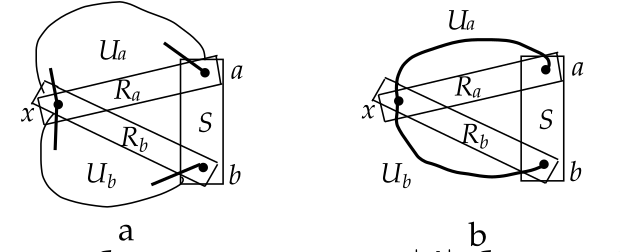
\includegraphics[width=0.5\columnwidth]{figures/theorem_2_1.png}
	\caption{Рисунок к Теореме \ref{theorem:2_1}.}
    \label{fig:theorem_2_1}
\end{figure}

	Переход: пусть $H = G(A)$, опять же по лемме \ref{lemma:2_3} $H$ имеет точку сочленения $x$, отделяющую $a$ от $b$.
	Пусть $U_a$ и $U_b$ компоненты связности графа $H - x$, содержащие $a$ и $b$ соответственно.
	Заметим, что других компонент в $H - x$ нет, ведь т.к. $x$ отделяет $a$ от $b$, то третья компонента $H - x$ была бы и в графе $G - x$, а он двусвязный.

	Обозначим $U_a' = U_a \setminus \{a\}$, тогда если $U_a' = \varnothing$, то тогда есть ребро  $xa$ и  $G(U_a \cup \{x\})$ это простой путь.
	Теперь считаем $U_a' \neq \varnothing$.
	Тогда $R_a = \{a, x \}$ отделяет $U'_a$ от остальных вершин в графе $G$.
	Потому что $x$ отделяет от $U_b'$, а во все остальные(не из $A$) можно попасть только пройдя по $a$ либо по $b$, но $x$ также отделяет $U_a'$ и от $b$.

	Тогда, по предположению индукции граф $G(U_a' \cup R_a) = G(U_a \cup \{x\})$ — простой путь $ax$.

	Аналогично $G(U_b \cup \{x\})$ простой путь $bx$.

	А следовательно и $G(A)$ простой путь $ab$.
\end{proof}

\subsection{Основная теорема о дереве разбиения двусвязного графа (каждая часть двусвязного графа — блок или цикл, расположение неодиночных разделяющих множеств двусвязного графа).}

\begin{customthm}{2.2} \label{theorem:2_2}
	Пусть $G$ - двусвязный граф.
	Тогда выполняются следующие утверждения:

	\begin{enumerate}
		\item Каждая часть $\Part(G)$ ~--- 3-блок или цикл
		\item Множество $R = \{a, b\}$ не одиночное множество из $\R_2(G) \iff a$ и $b$ - не соседние в циклическом порядке вершины некоторой части-цикла.
	\end{enumerate}

\end{customthm}

\begin{proof}
	\begin{enumerate}
		\item Пусть $A \in \Part(G)$.
			Из Леммы \ref{lemma:1_2} следует что $G'(A)$ двусвязный.

			Предположим, что $\exists S \in \R_2(G'(A))$.
			По Лемме \ref{lemma:1_2} тогда $S \in \R_2(G)$.
			Множество $S$ не может быть одиночным в $G$, т.к. разделяет часть $A \in \Part(G)$.
			Тогда по Лемме \ref{lemma:2_2}, $S$ - не одиночное разделяющее множество в  $G'(A)$.

			Следовательно, в  $G'(A)$ нет одиночных множеств.
			Тогда по теореме \ref{theorem:2_1} $G'(A)$ - цикл(тогда $A$-цикл) или трёхсвязный граф(тогда $A$ - 3-блок).

		\item $\Longleftarrow$. Пусть  $A = \{ a_1, a_2, \ldots, a_k \} \in \Part(G)$, причем вершины указаны в циклическом порядке, $R = \{a_1, a_m\}$, где  $2 < m < k$.

			Тогда  $R \in \R_2(G'(A))$ и делит граф  $G'(A)$ ровно на две части:

			\begin{align*}
				U_1 &= \{a_1, a_2, \ldots, a_m\} && U_2 = \{a_m, a_{m+1}, \ldots, a_k, a_1\}
			\end{align*}

			По Лемме \ref{lemma:1_2} имеем $R \in \R_2(G)$.

			И множество $R$ не одиночное т.к. можно взять пару вершин в $U_1, U_2$ отличных от $a, b$, которое будет разделять $R$.

			$\Longrightarrow$. Возьмем не одиночное множество $R$, оно в любом случае независимо со всеми одиночными множествами графа  $G$, тогда $R$ лежит в одной из частей $A \in \Part(G)$.

			По Лемме \ref{lemma:2_2} тогда $R \in \R_2(G'(A))$.

			Тогда $A$ не трёхсвязно, а значит по первому пункту $A$ - цикл длины хотя бы $4$.

			Следовательно  $R$ состоит из двух не соседних вершин этого цикла(иначе $R$ было бы одиночным).

	\end{enumerate}
\end{proof}


\begin{customcrly}{2.1} \label{corollary:2_1}
	Пусть $G$ - двусвязный граф, $R \in \R_2(G)$. Тогда $R$ не содержит внутренних вершин частей-блоков и частей-треугольников(т.е. частей-циклов длины 3) графа $G$.
\end{customcrly}
\begin{proof}
	Пусть $B \in \Part(G)$ - 3-блок или треугольник.
	Если  $R$ - одиночное множество и $x \in R \cap B$, то $x \in \Bound(B)$(ведь мы разбиваем граф $G$ множеством $\D(G)$).
	
	Если  $R$ - не одиночное, то $R \cap \Int(B) = \varnothing$ по Теореме \ref{theorem:2_2}.
\end{proof}

\begin{customcrly}{2.2} \label{corollary:2_2}
	Если часть $A \in \Part(G)$ - цикл, то все вершины из  $\Int(A)$ имеют степень 2 в графе $G$.
\end{customcrly}
\begin{proof}
	Если $x \in \Int(A)$, то рёбра графа $G$ выходят из $x$ только к вершинам части  $A$.
	А таких ребра всего два.
\end{proof}

\subsection{Части и подразбиение. Теорема Маклейна о планарности двусвязного графа.}

\begin{df*}[Подразбиение]
	Граф $H'$ называется \textbf{подразбиением} графа $H$, если  $H'$ может быть получен из  $H$ заменой некоторых рёбер на простые пути.
	Все добавляемые вершины различны и имеют степень 2. 

	Вершины графа $H'$, являющиеся вершинами графа  $H$(т.е. не являющиеся внутренними вершинами добавленных путей), называются \textbf{главными}.
\end{df*}

\begin{prop*}
	Через $G \supset H$ будем обозначать, что граф  $G$ содержит в качестве подграфа подразбиение графа  $H$.
\end{prop*}

\begin{customlm}{2.4} \label{lemma:2_4}
	Пусть $G$ - двусвязный граф,  $A \in \Part(G)$.
	Тогда  $G \supset G'(A)$.
\end{customlm}
\begin{proof}
	Пусть $ab \in E(G'(A)) \setminus E(G)$.
	Тогда  $a, b \in A$ и  $\{a, b\} \in \D(G)$. 

	Пусть $U_{a, b} \in \Part(\{a, b\})$ - часть, не содержащая $A$.

	Тогда существует  $ab$-путь $S_{a, b}$ по вершинам части  $U_{a, b}$ в графе $G$(потому что часть $S_{a, b}$ связна в $G$).
	Заменим ребро  $ab$ на этот путь  $S_{a, b}$ (т.е. мы как бы вместо одного прямого ребра $ab$ сделали длинный ребро-путь по вершинам не из $A$).

	Надо теперь показать что если так сделать для всех пар $ab \in E(G'(A)) \setminus E(G)$, то добавленные пути не будут пересекаться.

\begin{figure}[ht]
    \centering
	\incfig[0.4]{lemma_2_4}
	\caption{Пояснение к Лемме \ref{lemma:2_4}}
    \label{fig:lemma_2_4}
\end{figure}

	В результате нескольких таких замен мы получим подграф $H$ графа  $G$.
	Пусть $ab$ и  $xy$ два разных замененных ребра(возможно они имеют общий конец).
	Тогда части  $U_{a, b}$ и  $U_{x, y}$ разделены частью  $A$ в  $\BT(G)$, поэтому не имеют общей внутренней вершины.

	Следовательно, никакие два добавленных пути не имеют общей внутренней вершины, а значит, граф $H$ является подразбиением  $G'(A)$.

\end{proof}


\begin{remrk}[Теорема Понтрягина — Куратовского] \label{remark:pontyagin_kuratowski}
	Граф планарен тогда и только тогда, когда он не содержит подразбиений полного графа с пятью вершинами $K_5$ и полного двудольного графа с тремя вершинами в каждой доле $K_{3,3}$.
\end{remrk}

\begin{customthm}{2.3}[S. MacLane, 1937] \label{theorem:2_3}
	Пусть $G$ - двусвязный граф, а  $G' = G^{\D(G)}$.

	Тогда граф  $G$ планарен $\iff$ для любого 3-блока  $B \in \Part(G)$, граф  $G'(B)$ планарен.
\end{customthm}

\begin{proof}
	$\Longleftarrow$. Т.к. цикл планарен, то граф $G'(B)$ планарен просто для любой части  $B \in \Part(G)$.

	Пусть весь граф $G$ не планарен. Тогда по Замечанию \ref{remark:pontyagin_kuratowski} граф  $G$ имеет подграф  $H$ ~-- подразбиение  $K_5$ или  $K_{3,3}$.

	Пусть $M$ - множество главных вершин  $H$.

	Поскольку и $K_5$ и  $K_{3,3}$ трёхсвязны, то любое двухвершинное разделяющее множество графа  $H$ не разделяет $M$.
	Поэтому существует часть  $B \in \Part(G)$, что  $B \supset M$.

\begin{figure}[ht]
    \centering
	\incfig[0.4]{theorem_2_3}
	\caption{Пояснение к первому пункту доказательства Теоремы \ref{theorem:2_3}}
    \label{fig:theorem_2_3}
\end{figure}

	Предположим, что существует вершина $x \in V(H)$, что  $x \not \in B$.
	А значит вершина $x$ лежит на пути  $S_{a, b}$ для каких то главных вершин $a, b \in B$.

	Пусть $x \in A \in \Part(G)$.
	Т.к. $\BT(G)$ - дерево, то существует смежное с  $B$ в  $BT(G)$(т.е. входящее в границу $B$) одиночное множество $R = \{y, y'\}$, отделяющие $A$ от  $B$.

	Тогда если мы пойдем по пути  $S_{a, b}$ от  $x$ в обе стороны, мы попадем в вершины множества  $R$.
	Тогда можно заменить участок пути между  $y, y'$ на ребро $yy'$ графа  $G'$.
	После нескольких таких операций вершины вне части  $B$ закончатся и мы получим граф  $H'$ - подразбиение  $K_5$ или  $K_{3,3}$ вершины которого лежат в  $B$.

	А т.к.  $H'$ - подграф  $G'(B)$, то значит  $G'(B)$ не планарен. Противоречие.

	 $\Longrightarrow$. Пусть  $G'(B)$ не планарен.
	 По Лемме \ref{lemma:2_4} существует подграф  $H$ графа  $G$, являющийся подразбиением  $G'(B)$.
	 Значит и  $H$ не планарен, а значит и  $G$.

\end{proof}

\subsection{Критические двусвязные графы.}

\begin{df*}[Критический двусвязный граф]
	Назовем двусвязный граф  $G$ \textbf{критическим}, если он  теряет двусвязность при удалении любой вершины.
\end{df*}

\begin{customcrly}{2.3.1} \label{corollary:2_3_1}
	Двусвязный граф $G$ является критическим  $\iff$ все его части-блоки и части-треугольники имеют пустую внутренность.
\end{customcrly}

\begin{proof}
	По Теореме \ref{theorem:2_2} вершины, не входящие в множества из $\R_2(G)$(т.е. удаление которых не нарушает двусвязность графа $G$) - это как раз внутренние вершины 3-блоков и треугольников графа $G$.
	Ведь при удалении вершины из цикла длины  $4$ мы точно сделаем его односвязным. 
\end{proof}

\begin{customcrly}{2.3.2} \label{corollary:2_3_2}
	Пусть $A \in \Part(S)$ - крайняя часть критического двусвязного графа $G$, смежная в $\BT(G)$ с одиночным множеством  $S$.
	Тогда  $A$ - цикл длины хотя бы 4 и все вершины  $A$, кроме двух вершин множества  $S$, имеют в графе  $G$ степень 2.
\end{customcrly}

\begin{proof}
	Т.к. $A$ - крайняя часть графа  $G$, то  $A$ - цикл длины хотя бы 4(ведь треугольник и 3-блок не распадутся при удалении $S$), а  $S$ состоит из двух соседних вершин этого цикла(Теорема \ref{theorem:2_2}).
	Остальные (хотя бы две) вершины $A$ - внутренние и по Следствию \ref{corollary:2_2} имеют степень 2 в графе  $G$.

\begin{figure}[ht]
    \centering
	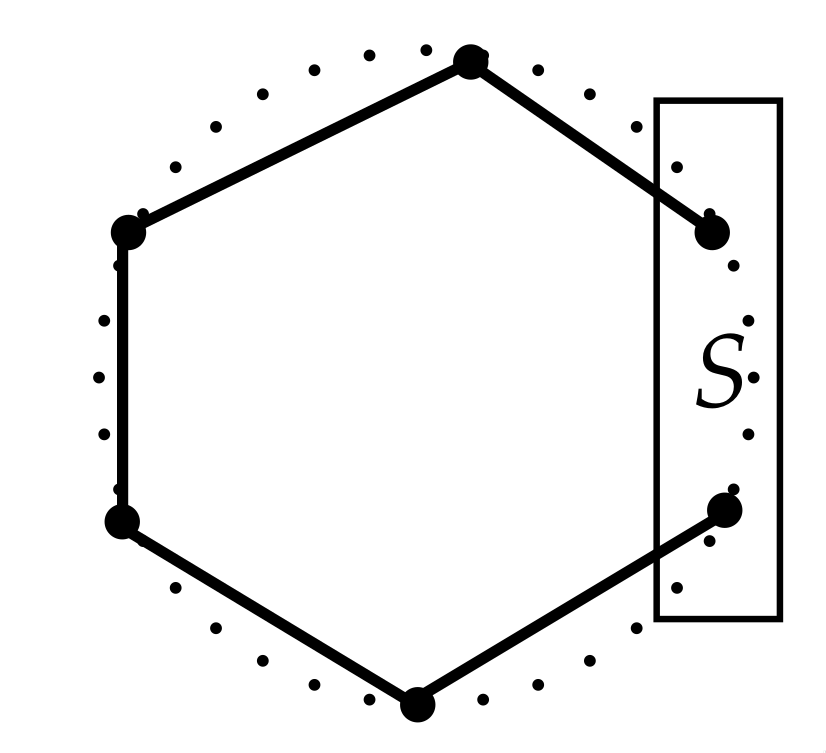
\includegraphics[width=0.2\columnwidth]{figures/corollary_2_3_2.png}
    \caption{Рисунок к Следствию \ref{corollary:2_3_2}}
    \label{fig:corollary_2_3_2}
\end{figure}

\end{proof}

\begin{crly}[Следствие 2.4, L. Nebesky, 1977] \label{corollary:2_4}
	Критический двусвязный граф $G : V(G) \geqslant 4$ имеет хотя бы 4 вершины степени ровно 2.
\end{crly}

\begin{proof}
	Если граф $G$ имеет хотя бы одно одиночное множество, то у него не менее двух крайних частей(одна часть это остаток цикла, а другая это просто какая то часть из оставшегося, содержащая $S$) и тогда по Следствию \ref{corollary:2_3_2} следует что у каждой такой части хотя бы две вершины степени 2.

	А если одиночных множеств в графе $G$ нет. То по Теореме \ref{theorem:2_1} этот граф либо трёхсвязен, либо простой цикл.
	Критический двусвязный граф, очевидно, не может быть трёхсвязным.
	А значит граф  $G$ это простой цикл на хотя бы 4х вершинах.
\end{proof}

\begin{claim*}
Заметим несколько фактор о критических двусвязных графах с 4 вершинами степени 2.

Если $|V(G)| = 4$, то это цикл на четырех вершинах.

Если  $|V(G)| > 4$, то это не цикл длины 5(ведь тогда было бы 5 вершин степени 2), а значит  $G$ содержит одиночные множества по Теореме \ref{theorem:2_1}.

Дерево $\BT(G)$ должно иметь ровно две висячие вершины(их не может быть меньше двух, т.к. в графе есть одиночное множество и не может быть больше двух, т.к. тогда будет слишком много вершин степени 2) и они соответствуют циклам длины 4(просто две вершины этого цикла лежат в одиночном множестве и их степень $> 2$).

Следовательно, все не крайние части и все одиночные множества имеют степень 2 в $\BT(G)$, т.к. $\BT(G)$ это просто путь между двумя частями-циклами.
Значит, каждое одиночное множество делит граф ровно на две части (для не одиночных множеств это всегда так).

Крайние части $G$(в объединении) содержат ровно 4 внутренних вершины степени 2, следовательно, в некрайних частях вершин степени 2 нет.

Пусть $A \in \Part(G)$ ~-- не крайняя часть.
Т.к. $\deg_{\BT(G)}(A) = 2$, то граница  $A$ состоит ровно из двух одиночных множеств, то есть, имеет 3 или 4 вершины.

Тогда $\Int(A) = \varnothing$, ведь если  $A$ ~-- 3-блок, то по Следствию \ref{corollary:2_3_1}, а если  $A$ ~-- цикл, то его внутренняя вершина имеет степень 2 в графе $G$, а таких в $A$ нет.

Таким образом, не крайняя часть $\Part(G)$ может быть треугольником, четырёхугольником или 3-блоком из четырёх вершин, причем ее вершины покрываются двумя одиночными множествами, смежными с этой частью в дереве $\BT(G)$.


\begin{figure}[ht]
    \centering
	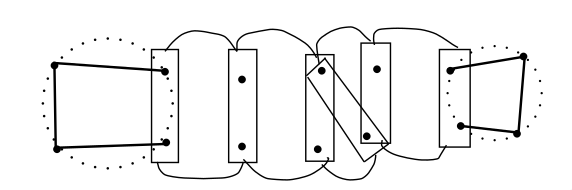
\includegraphics[width=0.4\columnwidth]{figures/example_2_critical_4_deg_2.png}
    \caption{Пример критического двусвязного графа $G$ с 4 вершинами степени 2.}
    \label{fig:example_2_critical_4_deg_2}
\end{figure}


\end{claim*}


\subsection{Теорема об удалении вершин из нескольких 3-блоков двусвязного графа.}

Если из связного графа удалить любую внутреннюю вершину, то он останется связным.

Более того, если удалить из связного графа множество, состоящее из нескольких внутренних вершин блоков и содержащее не более чем по одной вершине каждого блока, то связность сохранится.
Обобщим утверждение для двусвязного графа.

Следствие \ref{corollary:2_1} говорит нам, что вершина двусвязного графа, удаление которой не нарушает двусвязности - это внутренняя вершина части-блока или части треугольника.

\begin{remrk}[Теорема Менгера] \label{theorem:menger}
	Наименьшее число вершин, разделяющих две не смежные вершины $s$ и  $t$, равно наибольшему числу не пересекающихся простых $(s - t)$ цепей.
\end{remrk}

\begin{customthm}{2.4} \label{theorem:2_4}
	Пусть $G$ ~-- двусвязный граф, а $W$ - множество, состоящее из внутренних вершин не пустых 3-блоков графа  $G$ и содержащее не более чем по одной вершине из каждого 3-блока.
	Тогда граф  $G - W$ двусвязен.
\end{customthm}

\begin{proof}
	От противного, пусть $W$ - минимальное по включение множество, вершины которого принадлежат внутренностям разных не пустых 3-блоков, а граф  $G^* = G - W$ не двусвязен.
	Понятно, что  $|W| \geqslant 2$(ведь удаления одной вершины 3-блока недостаточно для нарушения двусвязности).

	Т.к. вершины  $W$ принадлежат внутренностям разных  $3$-блоков, то существует одиночное множество  $S = \{a, b\} \in \D(G)$, разделяющее  $W$(одиночное, потому что мы разбиваем семейством $\D(G)$).
	И тогда $S \cap W = \varnothing$(ведь все вершины из $W$ внутренние).
 
	Части $\Part(S)$ можно разбить на две группы так, чтобы в каждой группе была часть, содержащая вершину из  $W$.
	Пусть  $U_1$ и  $U_2$ - объединения вершин этих групп и 
	\[
		U^* = V(G) \setminus W = V(G^*), \qquad U_1^* = U_1 \setminus W, \qquad U^*_2 = U_2 \setminus W
	\]

	Т.к. каждый 3-блок графа $G$ содержит хотя бы 4 вершины(иначе это цикл) и не более чем одна из них лежит в  $W$, то:

	\[
		|U_1^*| \geqslant 3, \qquad |U_2^*| \geqslant 3
	\] 

	Положим:

	\[
		G_1^* = G(U_1^*), \qquad G_2^* = G(U_2^*), \qquad G_1 = G_1^* + ab, \qquad G_2 = G_2^* + ab
	\] 

	Пусть $x \in U_2 \cap W$.
	По минимальности $W$ получаем, что граф  $G_x = G - (W \setminus \{x\})$ двусвязен.

	Множество $S$ отделяет  $U_1^*$ от  $U_2^* \cup \{x \}$ в двусвязном графе $G_x$.
	По Лемме \ref{lemma:1_2}(для набора из одного множества $S$) граф $G_1$ двусвязен.
	Аналогично,  $G_2$ двусвязен.

	От любой вершины  $y \in U^*$ в графе  $G^*$ существует  $ya$-путь  $P_a$ и  $yb$-путь  $P_b$ не имеющие общих вершин, кроме  $y$(по теореме Менгера \ref{theorem:menger} для двусвязного графа  $G_1$ или $G_2$, в зависимости от расположения $y$). 

	Нам достаточно доказать, что \textit{для любой вершины $v \in U^*$ в графе  $G^* - v$ все вершины  $U^* \setminus \{v\}$ связаны}(т.е. что выкидывание любой вершин оставляет граф связным, значит он он двусвязен).

	Рассмотрим любую вершину $u \in U^* \setminus S$.
	В графе  $G^*$ существует два не пересекающихся пути от  $u$ до вершин множества  $S$(т.е до $a$ и  $b$).
	Один из этих путей есть и в  $G^* - v$.

	Остается доказать, что при  $v \not \in S$ вершины  $a$ и  $b$ множества  $S$ связаны в графе  $G^* - v$(из этого следует, что из всех вершин $U^*$ есть путь до $a$ или $b$ и при этом есть  $ab$-путь).
	Без ограничений общности, $v \in U_1^*$.
	Тогда существует $ab$-путь $P$ в графе $G^* - v$, проходящий по вершинам из $U_2^*$, значит, $a$ и $b$ связаны в  $G^* - v$.

	Значит $G^*$ двусвязен, противоречие предположению.
	Следовательно, граф $G - W$ двусвязен для любого множества $W$, удовлетворяющего условию.
\end{proof}

\subsection{Минимальные двусвязные графы.}

\begin{df*}[Минимальный двусвязный граф]
	Граф $G$ называется \textbf{минимальным двусвязным}, если он двусвязен и теряет двусвязность при удалении любого ребра.
\end{df*}

\begin{customthm}{2.5} \label{theorem:2_5}
	Двусвязный граф $G$ является минимальным тогда и только тогда, когда выполняются следующие условия:

	\begin{enumerate}
		\item Если $\{ a, b \} \in \R_2(G)$, то вершины  $a$ и  $b$ не смежны \label{cond:theorem_2_5_1}
		\item Для любого 3-блока $A$ графа $G$ граф $G(A)$ пуст(т.е. не имеет ни одного ребра) \label{cond:theorem_2_5_2}
	\end{enumerate}

\end{customthm}

\begin{proof}
	$\Longrightarrow$. Пусть  $G$ - минимальный двусвязный граф, проверим оба условия:

	\begin{enumerate}
		\item Предположим, что $S = \{a, b \} \in \R_2(G), \Part(S) = \{A_1, \ldots, A_n\}, ab \in E(G)$.

			Т.к. $G$ - двусвязен, то обе вершины $a$ и $b$ смежны с $\Int(A_j), \forall j \in [n]$.
			И граф  $G(\Int(A_j))$ связен, поэтому существует $ab$-путь, внутренние вершины которого лежат внутри  $\Int(A_j)$ для любого  $j \in [n]$. 

			Таким образом, в графе $G - ab$ существует  $n \geqslant 2$ не пересекающихся по внутренним вершинам  $ab$-путей.
			И значит в целом, между любой парой вершин найдется два не пересекающихся пути в графе $G - ab$. Ведь если при удалении одной вершины граф $G - ab$ разваливается, то значит  $a$ и $b$ должны попасть в разные компоненты связности(ведь при возвращении ребра $ab$ граф опять становится связным, значит достаточно проверить только их связность), но между ними выжил бы хотя бы один путь. Отсюда следует двусвязность графа  $G - ab$.

			Противоречие с минимальностью графа  $G$.

		\item Пусть $A$ ~-- 3-блок графа $G$;  $x, y \in A, xy \in E(G)$.

			Граф  $G'(A)$ ~-- трёхсвязен, следовательно, по теореме Менгера \ref{theorem:menger} существует три независимых  $xy$-пути в графе  $G'$. 

			По Лемме \ref{lemma:2_4} граф $G$ содержит подразбиение  $G'(A)$, поэтому в графе  $G$ также найдутся 3 не пересекающихся  $xy$-пути.
			Следовательно, в графе  $G - xy$ найдется хотя бы два  $xy$-пути, а значит, он двусвязен.

			Противоречие с минимальностью графа  $G$.
	\end{enumerate}

	$\Longleftarrow$. Покажем что для любого ребра $xy \in E(G)$ граф $G - xy$ не двусвязен.

	Т.к.  $x$ и  $y$ соединены ребром, то они обязательно лежат в одной части  $A \in \Part(G)$.
	Из условия \eqref{cond:theorem_2_5_2} и того что $xy \in E(G)$  следует, что  $A$ - цикл. 

	Пусть $z \in A \setminus \{x, y\}$.
	Тогда множество $T = \{z, xy\}$ - делит цикл $G'(A)$ на две компоненты связности:  $U_x, U_y$.

	Докажем, что  $x$ и  $y$ не связаны в графе  $G' - T$(это значит что после удаления ребра $xy$ граф  $G$ перестал быть двусвязным).

	От противного, пусть $P$ - кратчайший  $xy$-путь в  $G' - T$.

	Понятно, что  $V(P)$ содержит вершину $b \not \in A$(ведь $A$ распалось после удаления  $T$).
	Рассмотрим одиночное множество $S$, отделяющее  $b$ от  $A$(множество $S$ не равно  $\{x, y\}$, ведь по условию \eqref{cond:theorem_2_5_1} между вершинами  $S$ нет ребра).
	Т.к. $x, y \in A$, то при движении от  $b$ по пути  $P$ в сторону $x$ и  $y$ мы попадем в две разные вершины множества  $S$.
	Эти вершины смежны в  $G'$, тогда заменим участок пути  $P$, содержащий  $b$ на ребро  $e$ между двумя вершинами множества  $S$.
	Получим более короткий  $xy$-путь в графе $G'$.

	Т.к. $V(P') \subset V(P)$ и ребро  $e \not \in T$, путь $P'$ соединяет  $x$ с  $y$ и в графе  $G' - T$, противоречие с выбором пути  $P$.

	Следовательно, граф  $G - T$ не связен.


\end{proof}

\begin{df*}[$V_2(G)$]
	Для двусвязного графа $G$ обозначим  $V_2(G)$ - множество всех вершин степени ровно 2.
\end{df*}

\begin{df*}[$V_3(G)$]
	Для двусвязного графа $G$ обозначим  $V_3(G)$ - множество всех вершин степени хотя бы 3.
\end{df*}

\begin{customcrly}{2.5} \label{corollary:2_5}
	Пусть $G$ - минимальный двусвязный граф, тогда:

	\begin{enumerate}
		\item Если $A$ ~-- 3-блок графа  $G$, то  $\Int(A) = \varnothing$
		\item Пусть  $A$ ~-- крайняя часть графа  $G$. Тогда  $A$ ~-- цикл 
		\item Множество  $V_3(G)$ состоит из всех вершин, входящих в одиночные множества графа  $G$.
		Множество  $V_2(G)$ состоит из всех внутренних вершин частей графа  $G$(понятно, что вершин степени менее двух в графе $G$ нет)
	\end{enumerate}

\end{customcrly}

\begin{proof}
	\begin{enumerate}
		\item Пусть $x \in \Int(A)$, тогда рассмотрим произвольное ребро  $xy \in E(G)$, понятно что  $y \in A$(Теорема \ref{theorem:0_1}).
			Противоречие с Теоремой \ref{theorem:2_5}.
		\item Т.к. $A$ - крайняя часть, то $|A| > 2$ и при этом  $|\Bound(A)| = 2$, значит $\Int(A) \neq \varnothing$, значит из пункта 1 получаем что $A$ ~-- цикл.
		\item  Пусть $v \in \Int(A)$ для какой то части $A \in \Part(G)$.
			Тогда по пункту 1 получаем что $A$ - цикл.
			А следовательно  $d_G(v) = 2$, ведь $v \in \Int(A)$.

			А если $v$ входит в какое то одиночное множество и $\deg_G(v) = 2$, то тогда это множество не одиночное ведь можно отделить его через  $\N_G(v)$.
	\end{enumerate}
\end{proof}


